\documentclass[12pt]{extarticle}
\usepackage[utf8]{inputenc}
\usepackage[english]{babel}

\usepackage[disable]{todonotes}
\newcommand{\dg}[1]{\todo[inline]{DG: #1}}

\usepackage{xcolor}
\usepackage{wrapfig}

% Pollock
\definecolor{C0}{HTML}{000000}
\definecolor{C1}{HTML}{511818}
\definecolor{C2}{HTML}{3b4666}
\definecolor{C4}{HTML}{a04540}

\usepackage[%
% hidelinks,
%	bookmarksopen=true,
colorlinks=true,
%	citebordercolor={1 0 0},
%	citecolor=red,
% urlbordercolor={0 0 1},
urlcolor=C2%
]{hyperref}
% \urlstyle{same}
\usepackage[inline]{enumitem}
\usepackage[a4paper, top=2.5cm, bottom=2.5cm, left=2.1cm, right=2.1cm]{geometry}
\usepackage{microtype}

% A font combination which does not scream LaTeX
\usepackage{tgpagella}
\usepackage{eulervm}

\usepackage{setspace}

% Reduce figure space
% \renewcommand\floatpagefraction{.9}
% \renewcommand\topfraction{.9}
% \renewcommand\bottomfraction{.9}
% \renewcommand\textfraction{.1}
% \setcounter{totalnumber}{50}
% \setcounter{topnumber}{50}
% \setcounter{bottomnumber}{50}

% \makeatletter
% \renewcommand{\section}{\@startsection{section}{1}{0mm}
% {1.0\baselineskip}%
% {0.2\baselineskip}%
% {\normalfont\large\bfseries}}%
% \makeatother
% 
% \makeatletter
% \renewcommand{\subsection}{\@startsection{subsection}{2}{\z@}%
% {0.4\baselineskip}%
% {0.5ex \@plus .2ex}{\normalfont\normalsize\bfseries}}%
% \makeatother
% 
% \makeatletter
% \renewcommand{\subsubsection}{\@startsection{subsubsection}{3}{\z@}%
% {0.4\baselineskip}%
% {0.5ex \@plus .2ex}{\normalfont\normalsize\bfseries}}%
% \makeatother

% \renewcommand{\baselinestretch}{1.5}

\newcommand*\sq{\mathbin{\vcenter{\hbox{\rule{.8ex}{.8ex}}}}}
\newcommand*\ssq{\mathbin{\vcenter{\hbox{\rule{.6ex}{.6ex}}}}}
\newenvironment{t_sq_itemize}
{\begin{itemize}[topsep=0pt, parsep=0pt, itemsep=0pt, leftmargin=*]
    \renewcommand{\labelitemi}{{\(\sq\)}}}
  {\end{itemize}}

\begin{document}\color{C0}

\noindent
To: Natasha Timofeyuk \\
Chair of the European Research Committee \\
on Few-Body Problems in Physics

\bigskip\bigskip

\noindent
\doublespacing
{\color{C4}\fontfamily{qag}\selectfont%
  \LARGE Proposal for the\newline 26th
  European Few-Body Conference\newline
  to be held in Prague, Czech Republic%
}

\bigskip
% \renewcommand{\baselinestretch}{1.5}

\onehalfspacing
\section*{Venue and Host Institutions}
\noindent
%
The Conference will take place at the
\href{https://www.mff.cuni.cz/en}{Faculty of Mathematics and Physics},
\href{https://cuni.cz/UKEN-1.html}{Charles University} (Troja Campus,
V Holešovičkách 747/2, Praha 8) and will be hosted by
\href{http://www.ujf.cas.cz/en/}{Nuclear Physics Institute} of the
\href{https://www.avcr.cz/en/}{Czech Academy of Sciences} (ÚJF, Řež)
and Faculty of Mathematics and Physics, Charles University (MFF UK,
Prague).

% Jenom příklad
\begin{wrapfigure}[10]{r}{0.5\textwidth}
  \centering
  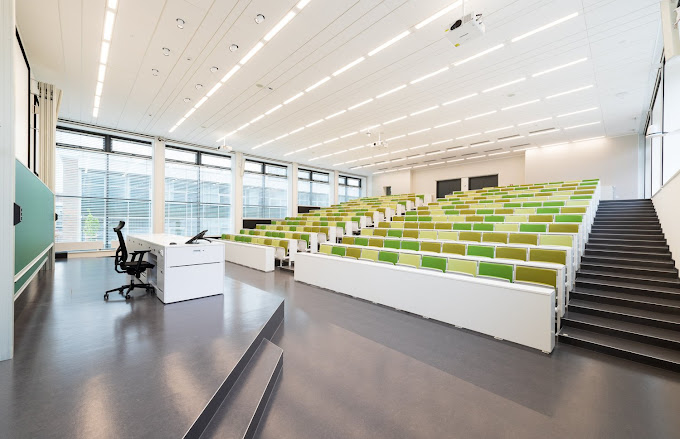
\includegraphics[width=0.48\textwidth]{Impakt-troja_1}
\end{wrapfigure}

\textbf{Charles University} (Latin: Universitas Carolina) is the oldest and
largest university in the Czech Republic. It is one of the oldest
universities in Europe in continuous operation.
% 
\textbf{The Czech Academy of Sciences} is the leading non-university public
research institution in the Czech Republic. Its tradition goes back to
the Royal Bohemian Society of Sciences founded in 1784. The Academy
conducts both fundamental and strategic applied research. The
  Nuclear Physics Institute of the Czech Academy of Sciences, a
public research institution, conducts research in a broad field of
nuclear physics, experimental as well as theoretical.
%
\textbf{Prague} with its rich history and stunning architecture is one of the
world's most popular tourist destinations. It is classified as an
``Alpha-{}'' global city according to GaWC studies. Prague ranked sixth
in the Tripadvisor world list of best destinations in 2016 (fifth in
2014). Furthermore, the city was ranked 7th in the world ICCA
Destination Performance Index measuring performance of conference
tourism in 2021.


\section*{Travel}
\noindent
%
Due to its location in the heart of Europe, Prague is easily
accessible. The most popular ways of getting to Prague are by plane or
by train. Prague has an extensive public transport network that is
rated as one of the best and most reliable in Europe.

{\bf Troja Campus, transport:} It is possible to travel to Troja by public transport, the closest bus stops being “Kuchyňka”
and “Pelc Tyrolka”. Alternatively, the campus is about 15 minutes walk from the metro station “Nádraží Holešovice”
(line C). It is also possible to drive to the campus by car. It is possible to park in front of the main entrance or in the courtyard;
parking is free and accessible nonstop.


\section*{Local Organizing Committee (preliminary)}
\noindent
The conference will be organized by a mixed committee of scientists from ÚJF, Řež and MFF UK, Prague.
The local organizing committee will include:
\begin{t_sq_itemize}
\item Nina Shevchenko, chair (ÚJF, Řež; theory)
\item Daniel Gazda (ÚJF, Řež; theory)
\item Tomáš Dytrych (ÚJF, Řež; theory)
\item Zdeněk Doležal (MFF UK, Prague; experiment)
\item Jiří Mareš (ÚJF, Řež; theory) 
\end{t_sq_itemize}

\section*{International Advisory Committee and time schedule}
\noindent
%
Members will be chosen from the lists of advisors from past conferences. New names
will be added in consultation with the European few-body research committee to ensure that all
areas of few-body research are covered. 

We assume to set the IAC to (datum), they will be asked to suggest the invidet speakers in (datum). 
The first announce about the EFB26 conference will be done in the autumn 2024, the web page
should be already ready at that time.

\section*{Topics}
\noindent
The following topics will be covered at the conference:
\begin{t_sq_itemize}
\item Nuclei and hypernuclei
\item Hadron physics
\item Electroweak processes
\item Nuclear astrophysics
\item Cold atoms and quantum gases
\item Atoms and molecules
\item Few-body methods
\item Few-body aspects of many-body systems
\end{t_sq_itemize}

\section*{Scientific program}
\noindent
We will maintain the traditional structure of few-body conferences lasting 5 days, from Monday
to Friday. We will leave Wednesday afternoon for excursion and/or discussions. We will have plenary sessions
in the mornings and parallel sessions in the afternoons. There will be about 30 plenary talks lasting
30 minutes, including the talks by young researcher awardees. Depending on the total number of
participants we will have either two or three parallel sessions. We will have a poster session as well.
We also plan to host a public lecture of general interest for participants and the public on a topic related
to the conference theme. 

\section*{Social program}
\noindent
Social program will include a welcome reception (at MFF UK), conference dinner (in the Prague center). 
We also will organize Prague city center excursion and excursions to ÚJF / MFF UK laboratories.

\section*{Registration fee will include}
\noindent
Conference kit, coffee breaks, lunches, welcome reception, conference dinner, excursions. Early bird registration fee, 20\%
reduced fee for students. No on-line participants are planned.
Lunches (preliminary): at Menza Troja (Pátkova 3, Praha 8), in walking distance from the conference place.

Fee for an accompanying person will include welcome reception and the conference dinner (?).

{\bf Plus:} Meeting rooms,  audio visual equipment,  free WiFi(?).


\section*{Budget}
\noindent
We assumed 150 participants, among them 30 students in estimating the conference fee.
A possibility to  get some extra funding is not too high, there are no special grants for conferences
in Czech Republic. However, we will use any other emerging opportunity to apply for the conference
support, thereby reducing the fee and making support possible for those with special circumstances.

We show our estimates in the Table below which includes both lower and higher estimates. The upper
estimate is calculated assuming a conservative possible rise of 20 \% in prices in three years time.  
CZK/EUR exchange rate (CZK = Czech koruna) will also play a role.

\begin{table}[h]
\centering
\begin{tabular}{ll}
\hline \\[-1mm]
 &   Price in CZK/EUR  \\[1mm]
\hline \\[-1mm]
 Full fee &  number \\[1mm]
 Early-bird fee & number  \\[1mm]
 Full student fee &  number \\[1mm]
 Early-bird student fee & number  \\[1mm]
 Accompanying person fee & number  \\[1mm]
\hline
\end{tabular}
\end{table}

\section*{Accommodation}
\noindent
Accommodation will not be included in the registration fee and must be organized by the participants.
Prague offers many possibilities for accommodation which can be found using usual booking portals. Close
to “Nádraží Holešovice” metro station are situated: Plaza Prague Hotel, Hotel Extol Inn Praha, Hotel Expo, Hotel
Castle Residence. We intend to arrange accommodation for reduced rates in selected hotels during the time of
the conference. The typical current costs per night ranges from about 75 EUR.

{\bf For students:} We plan to arrange and offer inexpensive accommodation at the nearby dormitory ``Kolej 17.
Listopadu - Univerzita Karlova'' (Pátkova 2136/3, Prague 8).

\section*{Other information}

\paragraph{Academic and Medical Conference Agency (AMCA)}
Services of AMCA will be used for registration, conference fee
collecting, book of abstract printing, catering, social dinner.

\paragraph{Visa}
Czech Republic does not require visas from EU/EEA citizens for stays
of any duration or for any purpose. Citizens of Australia, Brazil,
Canada, Israel, Japan, Mexico, New Zealand, South Korea, Taiwan, the
US and some other countries will also not require a visa for stays of
up to 90 days. Citizens of China, India, Iran, Pakistan, Russia, South
Africa, Turkey and some other countries require a visa. We will write
letters of invitation to those participants who need visas well in
advance and will recommend they apply for the visa well in advance.

\paragraph{Weather}
Daytime high temperatures in Prague tend to be around 24 ${}^\circ$C early in August but fall off to near
21-22 ${}^\circ$C near the month's end. A few of the warmer afternoons, especially early in August, can reach
up near 31 ${}^\circ$C.

\end{document}


%%%%%%%%%%%%%%%%%%%%%%%%%%%%%%%%%%%%%%%%
For one-column wide figures use syntax of figure~\ref{fig-1}
%\begin{figure}[h]
% Use the relevant command for your figure-insertion program
% to insert the figure file.
%\centering
%\includegraphics[width=1cm,clip]{tiger}
%\caption{Please write your figure caption here}
%\label{fig-1}       % Give a unique label
%\end{figure}

For figure with sidecaption legend use syntax of figure
%\begin{figure}
% Use the relevant command for your figure-insertion program
% to insert the figure file.
%\centering
%\sidecaption
%\includegraphics[width=5cm,clip]{tiger}
%\caption{Please write your figure caption here}
%\label{fig-3}       % Give a unique label
%\end{figure}
